

\section{Design and Implement of Malware IR System}

두 페이즈의 구조도는 Figure 과 같다. 두 페이즈에서 공통으로 존재하는 모듈은 Feature Extractor와 Neural Embedder 가 있다. 벡터 학습 페이즈에는 Classifier 가, 리트리벌 페이즈에는 랭킹 모듈이 포함되어있다. 
% Figure
\begin{figure}
  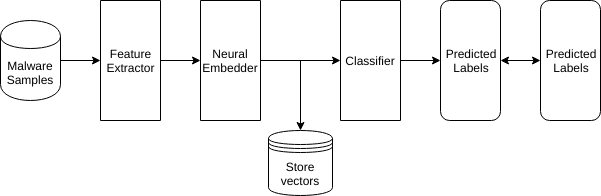
\includegraphics[width=\linewidth]{../figures/train_phase.png}
  \caption{train phase}
  \label{fig:one}
\end{figure}
% Figure
\begin{figure}
  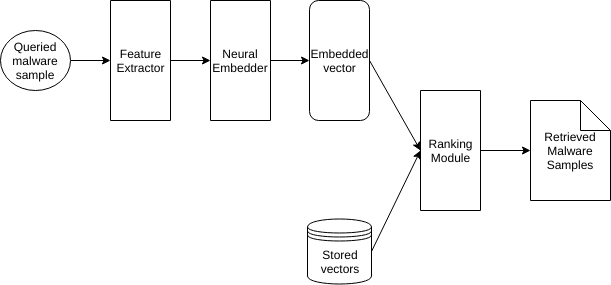
\includegraphics[width=\linewidth]{../figures/retrieval_phase.png}
  \caption{retrieval phase}
  \label{fig:two}
\end{figure}


\subsection{Feature Extractor}

Feature extractor 는 Malware Rawdata 로부터 Handcrafted feature 를 추출하는 모듈이다. Handcrafted feature로 PE 같은경우에는 Size 와 Entropy, Histogram of API Calls, … 등을[*] 추출한다. APK 같은 경우에는 추가적으로 Permission,  … 등의 피쳐를 추출한다. 


\subsection{Neural Embedder}
Neural embedder 는 Feature extractor 모듈에서 추출된 멀웨어의 피쳐들로부터 Representation vector 를 뽑는 모듈이다. theta 로 Parameterized 되어있는 뉴럴 네트워크이며, 파라미터는 벡터 학습 페이즈에서 Auxiliary Task 를 수행하면서 Optimize 된다. 그리고 리트리벌 페이즈에서 파라미터는 freeze 되어 업데이트되지 않는다. 

\subsection{Classifier}

classifier



